%LTeX: language=es-AR
\documentclass[
11pt, % The default document font size, options: 10pt, 11pt, 12pt
]{charter} 


% El títulos de la memoria, se usa en la carátula y se puede usar el cualquier lugar del documento con el comando \ttitle
\titulo{Predicción de riesgos financieros y estimaciones presupuestarias en construcción inmobiliaria con modelos de aprendizaje automático} 

% Nombre del posgrado, se usa en la carátula y se puede usar el cualquier lugar del documento con el comando \degreename
%\posgrado{Carrera de Especialización en Sistemas Embebidos} 
%\posgrado{Carrera de Especialización en Internet de las Cosas} 
\posgrado{Carrera de Especialización en Inteligencia Artificial}
%\posgrado{Maestría en Sistemas Embebidos} 
%\posgrado{Maestría en Internet de las cosas}

% Tu nombre, se puede usar el cualquier lugar del documento con el comando \authorname
% IMPORTANTE: no omitir titulaciones ni tildación en los nombres, también se recomienda escribir los nombres completos (tal cual los tienen en su documento)
\autor{Ing. Danilo Simón Reitano Andrades}

% El nombre del director y co-director, se puede usar el cualquier lugar del documento con el comando \supname y \cosupname y \pertesupname y \pertecosupname
\director{Dr. Ing. Hernán Garrido}
\pertenenciaDirector{Prof. Titular – FING, UNCUYO}

% Nombre del cliente, quien va a aprobar los resultados del proyecto, se puede usar con el comando \clientename y \empclientename
\cliente{Martin Brambati}
\empresaCliente{Built Technologies}
 
\fechaINICIO{29 de abril de 2025}		%Fecha de inicio de la cursada de GdP \fechaInicioName
\fechaFINALPlan{17 de junio de 2025} 	%Fecha de final de cursada de GdP
\fechaFINALTrabajo{30 de noviembre de 2024}	%Fecha de defensa pública del trabajo final


\begin{document}

\maketitle
\thispagestyle{empty}
\pagebreak


\thispagestyle{empty}
{\setlength{\parskip}{0pt}
\tableofcontents{}
}
\pagebreak


\section*{Registros de cambios}
\label{sec:registro}


\begin{table}[ht]
\label{tab:registro}
\centering
\begin{tabularx}{\linewidth}{@{}|c|X|c|@{}}
\hline
\rowcolor[HTML]{C0C0C0} 
Revisión & \multicolumn{1}{c|}{\cellcolor[HTML]{C0C0C0}Detalles de los cambios realizados} & Fecha      \\ \hline
0      & Creación del documento                                 &\fechaInicioName \\ \hline
1      & Se completa hasta el punto 5 inclusive                & 12 de mayo de 2025 \\ \hline
%2      & Se completa hasta el punto 9 inclusive
%		  Se puede agregar algo más \newline
%		  En distintas líneas \newline
%		  Así                                                    & {día} de {mes} de 202X \\ \hline
%3      & Se completa hasta el punto 12 inclusive                & {día} de {mes} de 202X \\ \hline
%4      & Se completa el plan	                                 & {día} de {mes} de 202X \\ \hline

% Si hay más correcciones pasada la versión 4 también se deben especificar acá

\end{tabularx}
\end{table}

\pagebreak



\section*{Acta de constitución del proyecto}
\label{sec:acta}

\begin{flushright}
Mendoza, \fechaInicioName
\end{flushright}

\vspace{2cm}

Por medio de la presente se acuerda con el \authorname\hspace{1px} que su Trabajo Final de la \degreename\hspace{1px} se titulará ``\ttitle'' y consistirá en el desarrollo un modelo de predicción de préstamos y presupuestos de construcción. El trabajo tendrá un presupuesto preliminar estimado de 600 horas y un costo estimado de \$ 1500, con fecha de inicio el \fechaInicioName\hspace{1px} y fecha de presentación pública a definir.

Se adjunta a esta acta la planificación inicial.

\vfill

% Esta parte se construye sola con la información que hayan cargado en el preámbulo del documento y no debe modificarla
\begin{table}[ht]
\centering
\begin{tabular}{ccc}
\begin{tabular}[c]{@{}c@{}}Dr. Ing. Ariel Lutenberg \\ Director posgrado FIUBA\end{tabular} & \hspace{2cm} & \begin{tabular}[c]{@{}c@{}}\clientename \\ \empclientename \end{tabular} \vspace{2.5cm} \\ 
\multicolumn{3}{c}{\begin{tabular}[c]{@{}c@{}} \supname \\ Director del Trabajo Final\end{tabular}} \vspace{2.5cm} \\
\end{tabular}
\end{table}




\section{1. Descripción técnica-conceptual del proyecto a realizar}
\label{sec:descripcion}

\subsection*{Introducción, contexto y propuesta de solución}

El presente trabajo surge a partir de una necesidad concreta de Built Technologies, empresa con sede en Nashville, Tennessee, Estados Unidos. Dicha necesidad de responder preguntas sobre los presupuestos de sus clientes fue identificada por el autor del documento, Danilo Reitano. Dicha empresa desarrolla una plataforma SaaS líder en la gestión de préstamos para la construcción. Trabaja con múltiples entidades bancarias y financieras que otorgan financiamiento a personas que planean construír su casa, desarrolladores y contratistas para la ejecución de proyectos residenciales y comerciales. La plataforma permite monitorear el uso del préstamo, la ejecución del presupuesto y los avances del proyecto de forma integrada.

Uno de los principales desafíos operativos que enfrenta la empresa, y en general el sector de préstamos para construcción, es la dificultad para validar en etapas tempranas si el importe del préstamo solicitado por el cliente será suficiente para cubrir los costos del proyecto. Actualmente, esta validación se realiza mediante revisiones manuales de los presupuestos enviados, que suelen estar desagregados en múltiples partidas (ej. cimentación, materiales, permisos, mano de obra, pisos, techos, terminaciones, etc.). Este proceso es altamente dependiente del criterio del analista y de las experiencias pasadas, sin una herramienta sistemática que permita predecir desvíos, subestimaciones o riesgos de insuficiencia presupuestaria. A menudo, estas deficiencias recién se manifiestan cuando el proyecto ya está en ejecución, mientras se generan sobrecostos, atrasos, renegociaciones contractuales o incluso abandono de obra.

En este contexto, la propuesta de esta tesis es el desarrollo de un sistema predictivo basado en modelos de aprendizaje automático que permita asistir de manera inteligente a los analistas de crédito en dos aspectos clave:

\begin{enumerate}
    \item Estimar, a partir de la información disponible al momento de analizar el préstamo, si el importe solicitado será suficiente para cubrir el presupuesto completo del proyecto.
    \item Predecir los costos esperados para cada una de las partidas presupuestarias del proyecto (por ejemplo: excavación, estructura, instalaciones eléctricas, techado, acabados). Se deberá tener en cuenta características del proyecto como su ubicación, tipo, proveedor, constructor, superficie y otros factores históricos.
\end{enumerate}

Este doble enfoque con distintas capas de análisis permitirá no solo detectar situaciones de riesgo financiero de manera temprana, sino también ofrecer recomendaciones concretas sobre los costos esperados. Todo esto en función de los datos históricos, ajustados al contexto de cada proyecto.

\subsection*{Contexto y condiciones particulares del proyecto}

Este proyecto se desarrollará en estrecha colaboración con el equipo de datos de Built Technologies. Se cuenta con acceso autorizado a un dataset anonimizado que incluye información detallada de más de 10 años de historial de proyectos, con datos por rubro presupuestario, tipo de préstamo, ubicación, resultados de ejecución y características del contratista y del proveedor. Por cuestiones de privacidad y cumplimiento normativo (SOC 2 y GDPR), los datos no contienen información sensible de clientes, y el trabajo se limita exclusivamente a información estructurada, sin el uso de documentos escaneados o imágenes.

\subsection*{Estado del arte y diferenciación de la solución}

En términos generales, existen diversas aplicaciones de modelos de machine learning en el ámbito financiero, particularmente en la evaluación de crédito, detección de fraude y puntuación de clientes. Sin embargo, el uso de aprendizaje automático para prever costos de construcción y validar la suficiencia de préstamos basándonos en presupuestos históricos es aún una línea de investigación y desarrollo incipiente.

La mayoría de las soluciones actuales en el sector se apoyan en heurísticas basadas en precios unitarios, bases de datos estáticas por región o \textit{benchmarking} manual entre proyectos. Esto tiene limitaciones evidentes: no contempla el contexto completo del proyecto ni aprende de los patrones reales de ejecución observados en los últimos años. Además, a medida que los proyectos modernos incrementaron en escala y complejidad, los métodos convencionales resultan insuficientes para capturar todas las variables que afectan los costos.

La regresión multivariada ha sido un enfoque base para estimar costos de construcción. Estos modelos asumen relaciones lineales entre los factores (como tamaño de la obra, calidad de los materiales, etc.) y el costo total. En escenarios relativamente simples, las regresiones pueden brindar estimaciones razonables: típicamente logran una precisión del orden de 75 \%-80 \%. No obstante, en la mayoría de proyectos existen relaciones no lineales y dependencias complejas entre variables (economías de escala, influencias del mercado, interacciones entre diseño y método constructivo) que limitan la capacidad predictiva.

También se ha explorado la utilización de otro tipo de modelos como \textit{Random Forest} y \textit{XGBoost}. Estos enfoques han mostrado mejoras significativas en precisión frente a métodos tradicionales. Por ejemplo, un estudio recopiló datos de 95 proyectos de edificios y implementó un modelo de \textit{Random Forest} para predecir riesgos de sobrecostos. Otro ejemplo relevante es un trabajo que utiliza \textit{XGBoost} para seleccionar las variables más influyentes y estimar el costo de proyectos de edificación.

En otros casos, se ha explorado la posibilidad de utilizar modelos de \textit{deep learning} para estimación de costos en el desarrollo de proyectos. Algunas investigaciones han resultado en precisiones del 85 \%-90 \%, superior a la obtenida por modelos más simples. Esto se traduce en menores errores de predicción para proyectos complejos, aunque a costa de una mayor demanda de datos y capacidad computacional.

Al leer los resultados de dichos proyectos, se puede apreciar que las variables de mayor influencia son la escala del proyecto (metros cuadrados construídos, número de plantas), funcionalidad (edificio residencial, comercial, salud, etc.), así como especificaciones técnicas principales (tipo de climatización, sistema estructural, acaados exteriores e interiores, presencia de elementos especiales como ascensores, etc.), ubicación geográfica, año o época de construcción y tipo de contrato, entre otros.


La solución propuesta se diferencia en que:
\begin{itemize}
    \item Utiliza modelos de aprendizaje supervisado entrenados sobre datos reales de ejecución y financiamiento, con ajuste de las predicciones al comportamiento histórico.
    \item Integra múltiples variables categóricas y numéricas, como ubicación geográfica, superficie construida, tipo de contratista y composición del presupuesto, con una predicción contextualizada.
    \item Utiliza un volumen de datos mayor a los proyectos realizados hasta el momento.
    \item Incorpora técnicas de explicabilidad como SHAP (Shapley Additive Explanations) para interpretar por qué el modelo predice insuficiencia o sobrecosto, con adopción por parte de analistas humanos.
    \item Ofrece tanto una salida binaria (¿es suficiente el préstamo?) como una salida regresiva multirrubro (estimación de costos por partida).
\end{itemize}

\subsection*{Propuesta de valor e impacto esperado}

La implementación de este sistema generará múltiples beneficios para Built Technologies y sus socios financieros:

\begin{itemize}
    \item Reducir el porcentaje de proyectos con préstamos insuficientes y así lograr evitar renegociaciones y sobrecostos.
    \item Mejorar la eficiencia del análisis crediticio, donde los analistas cuentan con una herramienta predictiva basada en datos.
    \item Aumentar la satisfacción del cliente final, sin interrupciones en la ejecución del proyecto por errores de estimación.
    \item Detectar patrones de subestimación crónica en ciertos rubros o regiones, lo que podría informar futuras políticas de originación de préstamos.
\end{itemize}

El sistema se implementará inicialmente como un prototipo funcional con salida en formato tabular y visual, para luego ser integrado en el flujo de trabajo de análisis crediticio mediante una API o módulo dentro de la plataforma existente.

\subsection*{Descripción funcional de la solución}

La solución se compone de los siguientes bloques funcionales:

\begin{itemize}
    \item \textbf{Módulo de extracción de datos}: identificación, scrapping y unificación de datos.
    \item \textbf{Módulo de procesamiento de datos}: limpieza, transformación y validación de los datos históricos estructurados.
    \item \textbf{Módulo de entrenamiento}: entrenamiento de dos modelos: uno de clasificación binaria (suficiencia del préstamo) y otro de regresión multirrubro (predicción de costos por partida).
    \item \textbf{Módulo de inferencia}: dado un nuevo proyecto con sus características, el sistema entrega predicciones de suficiencia y una tabla con los valores esperados por rubro presupuestario.
    \item \textbf{Módulo de visualización}: presenta los resultados a través de gráficos, tablas y explicaciones interpretables para el uso por parte del equipo financiero.
\end{itemize}

En la figura \ref{fig:diagBloques} se presenta el diagrama en bloques del sistema. Se observa el flujo de datos desde la base histórica, las etapas de preprocesamiento, entrenamiento e inferencia, hasta la visualización de resultados por parte del analista financiero.

\begin{figure}[htpb]
\centering 
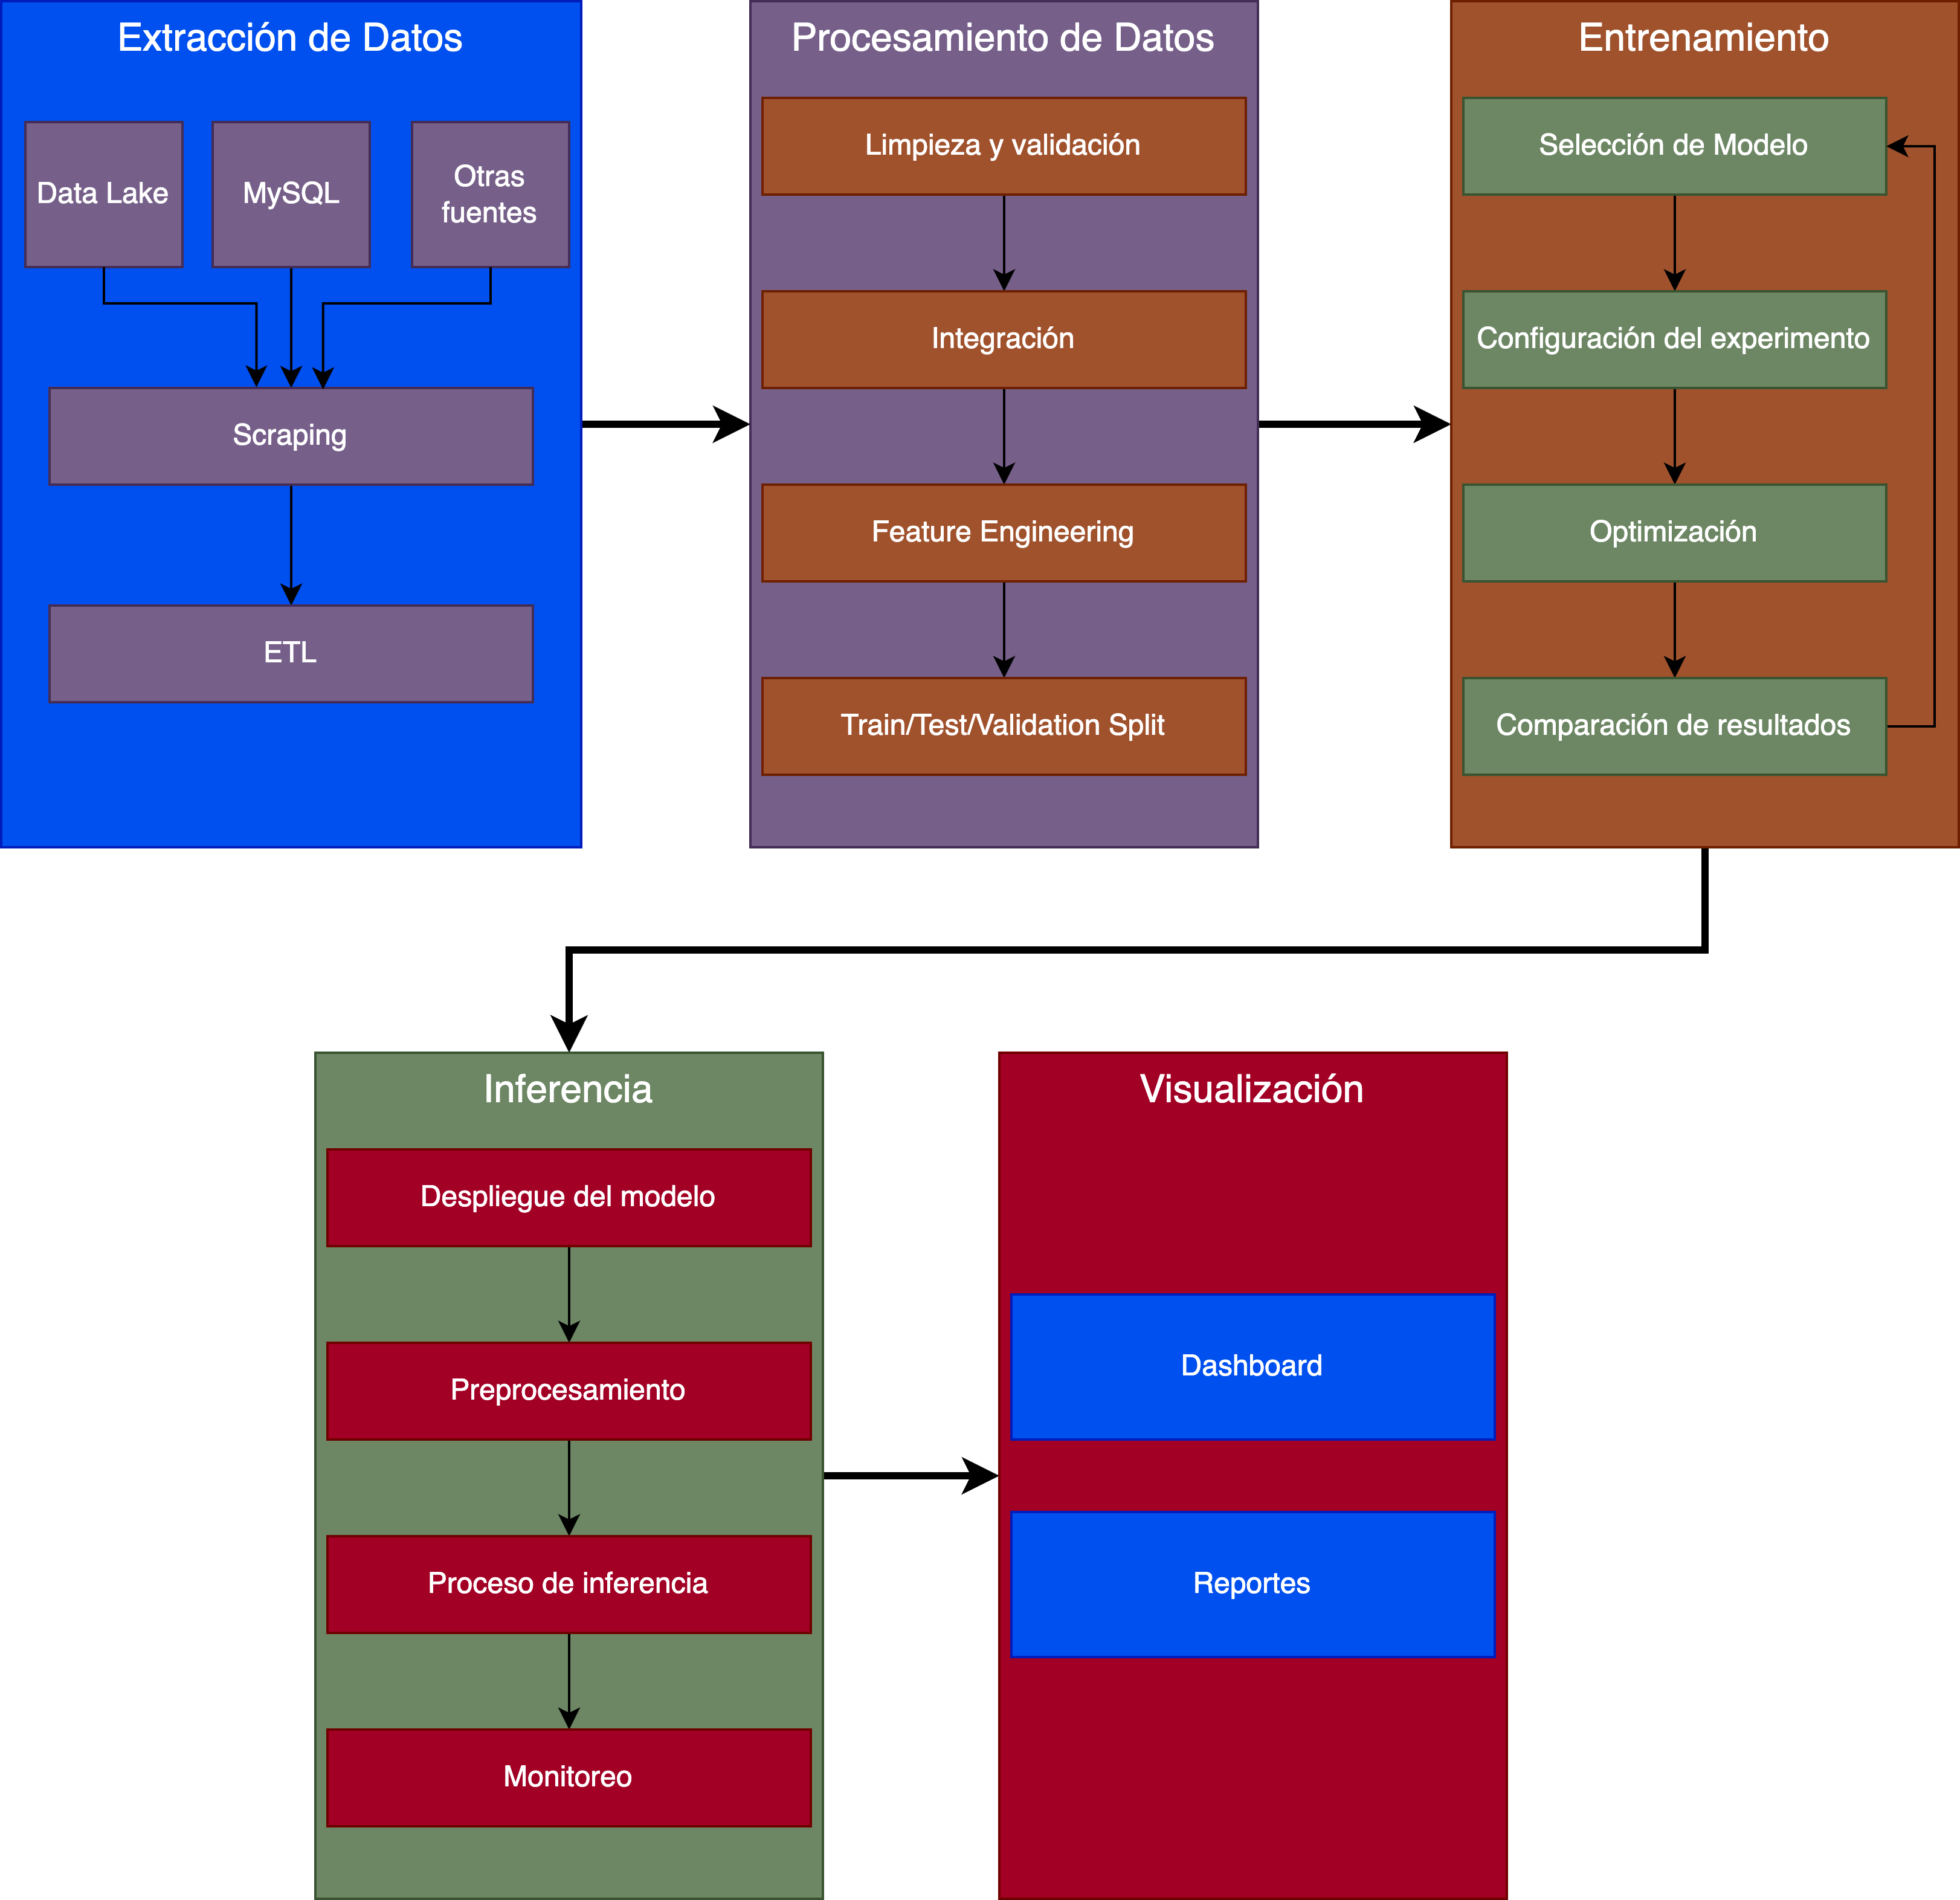
\includegraphics[width=1\textwidth]{./Figuras/bloques.png}
\caption{Diagrama en bloques del sistema.}
\label{fig:diagBloques}
\end{figure}

\section{2. Identificación y análisis de los interesados}
\label{sec:interesados}

\begin{table}[ht]
%\caption{Identificación de los interesados}
%\label{tab:interesados}
\begin{tabularx}{\linewidth}{@{}|l|X|X|l|@{}}
\hline
\rowcolor[HTML]{C0C0C0} 
Rol           & Nombre y Apellido & Organización         & Puesto \\ \hline
Cliente       & \clientename      &\empclientename       & Engineering Manager \\ \hline
Responsable   & \authorname       & FIUBA        	       & Alumno \\ \hline
Colaboradores & Thomas Schlegel   &\empclientename       & Distinguished Engineer	\\ \hline
Orientador    & \supname	        & \pertesupname 	     & Director del Trabajo Final \\ \hline
Opositores    & -                 & Procore Technologies & - \\ \hline
Usuario final & -                 & Clientes de Built 	 & - \\ \hline
\end{tabularx}
\end{table}

\begin{itemize}
	\item Orientador: a definir.
	\item Cliente: Martin Brambati posee una amplia trayectoria como mánager y director de ingeniería. Su experiencia será de gran valor para el desarrollo del proyecto.
	\item Colaboradores: Thomas Schlegel cuenta con más de 8 años de experiencia a cargo del área de datos en Built Technologies, lo que será de gran ayuda para la comprensión del conjunto de datos.
	\item Opositores: Procore Technologies proporciona una plataforma unificada de gestión financiera de proyectos de construcción. La empresa incorporó anteriormente herramientas de inteligencia artificial, por la que tendría intenciones de que este proyecto no llegue a concluirse.
\end{itemize}

\section{3. Propósito del proyecto}
\label{sec:proposito}

Desarrollar una solución basada en modelos de aprendizaje automático que permita asistir a los analistas financieros de Built Technologies en la evaluación de la suficiencia de préstamos otorgados para proyectos de construcción. Dicha solución deberá orientar en la estimación detallada de los costos asociados a cada una de las partidas presupuestarias. La solución busca anticipar riesgos de subfinanciamiento y sobrecostos mediante el análisis de datos históricos anonimizados. Esto produce decisiones más informadas, eficientes y escalables dentro del flujo de originación de créditos.

\section{4. Alcance del proyecto}
\label{sec:alcance}

El presente proyecto incluye:

\begin{itemize}
    \item Relevamiento y comprensión del problema de negocio asociado a la evaluación de suficiencia de préstamos y estimación presupuestaria en proyectos de construcción.
    \item Exploración, limpieza y transformación del conjunto de datos históricos anonimizados proporcionado por Built Technologies.
    \item Desarrollo de un pipeline de preprocesamiento de datos, que incluirá:
    \begin{itemize}
        \item Tratamiento de valores faltantes.
        \item Codificación de variables categóricas.
        \item Normalización y estandarización de variables numéricas.
        \item Balanceo de clases en caso de desbalance significativo en la variable objetivo (para el modelo de clasificación).
    \end{itemize}
    \item Entrenamiento y validación de:
    \begin{itemize}
        \item Un modelo de clasificación binaria para predecir si el préstamo solicitado es suficiente para cubrir el presupuesto total.
        \item Un modelo de regresión multivariada para estimar los costos esperados por categoría presupuestaria (por ejemplo: cimentación, electricidad, techado, etc.).
    \end{itemize}
    \item Evaluación de los modelos desarrollados mediante métricas adecuadas (\textit{F1-score}, \textit{AUC-ROC}, \textit{MAE}, \textit{RMSE}).
    \item Generación de explicaciones interpretables de las predicciones con técnicas como \textit{SHAP} o \textit{Feature Importance}.
    \item Documentación del proceso completo y presentación de los resultados en un formato replicable y académico.
\end{itemize}

El presente proyecto no incluye:

\begin{itemize}
    \item El desarrollo de una interfaz gráfica de usuario.
    \item La integración de los modelos desarrollados en los sistemas de producción de Built Technologies.
    \item La automatización completa del pipeline en un entorno de producción.
    \item La toma de decisiones finales sobre políticas de crédito, las cuales quedarán en manos del equipo financiero de la empresa.
    \item El análisis de documentos no estructurados.
\end{itemize}


\section{5. Supuestos del proyecto}
\label{sec:supuestos}


Para el desarrollo del presente proyecto se supone que:

\begin{itemize}
    \item El dataset estructurado y anonimizado proporcionado por Built Technologies estará disponible desde el inicio del proyecto, y contará con la calidad y cantidad suficientes para el entrenamiento de modelos de aprendizaje automático.
    \item No se requerirá solicitar acceso a datos sensibles o confidenciales.
    \item El alcance del proyecto se mantendrá centrado en el desarrollo de modelos predictivos (clasificación y regresión), sin requerir su integración en producción o implementación de interfaces visuales para usuarios finales.
    \item Se dispondrá de una dedicación mínima de 8 horas semanales para el proyecto a lo largo del año calendario 2025, con el propósito de compatibilizar las responsabilidades laborales con los tiempos del posgrado.
    \item Se contará con acceso continuo a recursos computacionales adecuados (principalmente Jupyter notebooks, Python y bibliotecas de ML como scikit-learn, XGBoost, pandas y SHAP), sin necesidad de infraestructura especializada ni servicios cloud pagos adicionales.
    \item Se contará con la disponibilidad del director del trabajo final para realizar revisiones metodológicas periódicas y seguimiento académico del progreso del proyecto.
\end{itemize}

\section{6. Product Backlog}
\label{sec:backlog}

El criterio utilizado para asignar los \textit{Story Points} se basa en una escala relativa de complejidad, esfuerzo y riesgo:
\begin{itemize}
  \item 1 punto: tarea simple, conocida, sin incertidumbre técnica.
  \item 2–3 puntos: tarea con un nivel medio de procesamiento o exploración de datos.
  \item 5 puntos: tarea técnica de mediana complejidad o con validaciones múltiples.
  \item 8+ puntos: tarea compleja o con alto nivel de incertidumbre en datos o rendimiento del modelo.
\end{itemize}

A continuación, se detallan las épicas y sus respectivas historias de usuario:

\begin{itemize}
  \item \textbf{Épica 1: planificación y organización del proyecto}
    \begin{itemize}
      \item \textbf{HU1:} Como responsable del proyecto, quiero definir un cronograma tentativo con fases y sprints para distribuir el trabajo de manera equilibrada.  
      \newline \textbf{Prioridad: Alta} — \textbf{Story Points: 3}

      \item \textbf{HU2:} Como estudiante, quiero actualizar y ajustar el backlog y el plan de trabajo según avances reales y obstáculos encontrados.  
      \newline \textbf{Prioridad: Media} — \textbf{Story Points: 2}
    \end{itemize}

  \item \textbf{Épica 2: relevamiento y análisis de datos históricos}
    \begin{itemize}
      \item \textbf{HU3:} Como analista de datos, quiero explorar y limpiar el \textit{dataset} histórico para asegurar que los datos sean utilizables para modelado.  
      \newline \textbf{Prioridad: Alta} — \textbf{Story Points: 3}
      
      \item \textbf{HU4:} Como ingeniero de datos, quiero identificar las variables más relevantes para el análisis, clasificándolas según tipo y calidad.  
      \newline \textbf{Prioridad: Alta} — \textbf{Story Points: 3}
    \end{itemize}

  \item \textbf{Épica 3: preprocesamiento y preparación de datos}
    \begin{itemize}
      \item \textbf{HU5:} Como científico de datos, quiero balancear las clases de la variable objetivo para asegurar un entrenamiento adecuado del modelo de clasificación.  
      \newline \textbf{Prioridad: Media} — \textbf{Story Points: 5}

      \item \textbf{HU6:} Como científico de datos, quiero normalizar y codificar las variables categóricas y numéricas para que puedan ser interpretadas por los modelos.  
      \newline \textbf{Prioridad: Alta} — \textbf{Story Points: 3}
    \end{itemize}

  \item \textbf{Épica 4: entrenamiento y validación de modelos}
    \begin{itemize}
      \item \textbf{HU7:} Como desarrollador de modelos, quiero entrenar un modelo de clasificación para predecir si los presupuestos cumplen con su objetivo, y evaluar su rendimiento con métricas como \textit{F1-score} y \textit{AUC}.  
      \newline \textbf{Prioridad: Alta} — \textbf{Story Points: 5}

      \item \textbf{HU8:} Como desarrollador de modelos, quiero entrenar un modelo de regresión para estimar los costos por partida presupuestaria, y analizar su precisión mediante \textit{MAE} y \textit{RMSE}.  
      \newline \textbf{Prioridad: Alta} — \textbf{Story Points: 5}
    \end{itemize}

  \item \textbf{Épica 5: interpretación, documentación y validación}
    \begin{itemize}
      \item \textbf{HU9:} Como analista, quiero aplicar técnicas de interpretabilidad (\textit{SHAP}, \textit{Feature Importance}) para entender las variables que más influyen en las predicciones.  
      \newline \textbf{Prioridad: Media} — \textbf{Story Points: 3}

      \item \textbf{HU10:} Como responsable del proyecto, quiero documentar el proceso, los resultados y sus limitaciones para facilitar su presentación y revisión académica.  
      \newline \textbf{Prioridad: Alta} — \textbf{Story Points: 2}
    \end{itemize}

  \item \textbf{Épica 6: sistematización y documentación técnica}
    \begin{itemize}
      \item \textbf{HU11:} Como autor del modelo, quiero documentar todas las decisiones de preprocesamiento y justificación de selección de variables para asegurar trazabilidad.  
      \newline \textbf{Prioridad: Alta} — \textbf{Story Points: 3}

      \item \textbf{HU12:} Como desarrollador, quiero versionar el código y registrar los experimentos de modelado para facilitar replicabilidad futura.  
      \newline \textbf{Prioridad: Media} — \textbf{Story Points: 3}
    \end{itemize}

  \item \textbf{Épica 7: redacción del trabajo final}
    \begin{itemize}
      \item \textbf{HU13:} Como alumno de posgrado, quiero redactar la memoria escrita del trabajo final, incorporando antecedentes, metodología, resultados y conclusiones.  
      \newline \textbf{Prioridad: Alta} — \textbf{Story Points: 8}

      \item \textbf{HU14:} Como autor, quiero adaptar el documento a los lineamientos formales de la universidad para asegurar su correcta presentación.  
      \newline \textbf{Prioridad: Alta} — \text8bf{Story Points: 3}
    \end{itemize}

  \item \textbf{Épica 8: preparación de la defensa oral}
    \begin{itemize}
      \item \textbf{HU15:} Como expositor, quiero preparar una presentación clara y visual para explicar el problema, la solución y los resultados a un jurado.  
      \newline \textbf{Prioridad: Alta} — \textbf{Story Points: 5}

      \item \textbf{HU16:} Como expositor, quiero ensayar la defensa oral para responder preguntas técnicas y asegurarme de cumplir con los tiempos estipulados.  
      \newline \textbf{Prioridad: Media} — \textbf{Story Points: 3}
    \end{itemize}
\end{itemize}

\section{7. Criterios de aceptación de historias de usuario}
\label{sec:criteriosAceptacion}

\begin{itemize}
  \item \textbf{Épica 2: relevamiento y análisis de datos históricos}
    \begin{itemize}
      \item \textbf{Criterios de aceptación HU3}
      \begin{itemize}
        \item El conjunto de datos ha sido cargado correctamente en el entorno de trabajo.
        \item Se identificaron y eliminaron valores atípicos y registros duplicados.
        \item Se generó un informe exploratorio con estadísticas descriptivas y visualizaciones básicas.
      \end{itemize}
      \item \textbf{Criterios de aceptación HU4}
      \begin{itemize}
        \item Se ha identificado el conjunto de variables relevantes para el modelo.
        \item Las variables han sido clasificadas como numéricas o categóricas.
        \item Se documentó la justificación técnica de la selección de cada variable.
      \end{itemize}
    \end{itemize}

  \item \textbf{Épica 3: preprocesamiento y preparación de datos}
    \begin{itemize}
      \item \textbf{Criterios de aceptación HU5}
      \begin{itemize}
        \item Se analizó la distribución de la variable objetivo y se detectó desbalance significativo (si aplica).
        \item Se aplicó una técnica de balanceo (\textit{undersampling}, \textit{oversampling} o \textit{SMOTE}).
        \item Se verificó que el modelo no pierda precisión tras aplicar balanceo.
      \end{itemize}
      \item \textbf{Criterios de aceptación HU6}
      \begin{itemize}
        \item Todas las variables categóricas han sido codificadas mediante \textit{one-hot encoding} o similar.
        \item Las variables numéricas fueron normalizadas o estandarizadas.
        \item El conjunto de datos final está listo para ser consumido por los modelos.
      \end{itemize}
    \end{itemize}

  \item \textbf{Épica 4: entrenamiento y validación de modelos}
    \begin{itemize}
      \item \textbf{Criterios de aceptación HU7}
      \begin{itemize}
        \item El modelo de clasificación fue entrenado con un conjunto dividido en entrenamiento, validación y prueba.
        \item Se reportan métricas \textit{F1-score} y \textit{AUC} en el conjunto de prueba.
        \item Se alcanza un \textit{F1-score} mayor al valor base definido como mínimo aceptable.
      \end{itemize}
      \item \textbf{Criterios de aceptación HU8}
      \begin{itemize}
        \item Se ha entrenado un modelo de regresión con variables de entrada preprocesadas.
        \item Se calculan métricas \textit{MAE}, \textit{RMSE} y \textit{R²} sobre el conjunto de prueba.
        \item El modelo logra un \textit{MAE} dentro del umbral definido según el negocio.
      \end{itemize}
    \end{itemize}

  \item \textbf{Épica 5: interpretación, documentación y validación}
    \begin{itemize}
      \item \textbf{Criterios de aceptación HU9}
      \begin{itemize}
        \item Se aplicó una técnica de explicabilidad (ej. \textit{SHAP}) sobre los modelos entrenados.
        \item Se identificaron las variables más influyentes en las predicciones.
        \item Los resultados de interpretabilidad se incluyen en un informe gráfico y textual.
      \end{itemize}
      \item \textbf{Criterios de aceptación HU10}
      \begin{itemize}
        \item Se generó un documento técnico con los pasos realizados, decisiones tomadas y resultados.
        \item El documento incluye gráficas de métricas y análisis de errores.
        \item El entregable final cumple con los requisitos formales del trabajo final académico.
      \end{itemize}
    \end{itemize}
\end{itemize}

\section{8. Fases de CRISP-DM}

\begin{enumerate}
  \item \textbf{Comprensión del negocio:}  
  El objetivo principal del proyecto es asistir a analistas financieros de Built Technologies mediante modelos predictivos que permitan:
  \begin{itemize}
    \item Estimar si el préstamo otorgado será suficiente para cubrir el presupuesto total de un proyecto de construcción.
    \item Predecir el costo esperado por categoría presupuestaria (materiales, mano de obra, cimentación, etc.).
  \end{itemize}
  El valor agregado de incorporar IA radica en anticipar riesgos de subfinanciamiento y sobrecostos desde etapas tempranas del proceso crediticio.  
  \textbf{Métricas de éxito:} precisión del modelo (\textit{F1-score} y \textit{AUC} para clasificación, \textit{MAE} y \textit{R²} para regresión), interpretabilidad y aplicabilidad práctica para el analista.

  \item \textbf{Comprensión de los datos:}  
  El dataset proviene de registros históricos anonimizados de Built Technologies, con más de 10 años de datos sobre proyectos financiados.  
  \begin{itemize}
    \item \textbf{Tipo:} datos estructurados tabulares, con variables numéricas y categóricas.
    \item \textbf{Origen:} base interna de proyectos y préstamos otorgados.
    \item \textbf{Cantidad:} en el orden de los millones de registros.
    \item \textbf{Calidad:} excelente, pero con presencia de valores faltantes, codificación inconsistente de categorías y posibles \textit{outliers}.
  \end{itemize}

  \item \textbf{Preparación de los datos:}  
  Esta etapa incluye limpieza y transformación del \textit{dataset} para su uso por los modelos:
  \begin{itemize}
    \item Eliminación de registros con errores evidentes o duplicados.
    \item Tratamiento de valores nulos mediante imputación o eliminación.
    \item Codificación de variables categóricas (\textit{one-hot encoding}).
    \item Normalización y estandarización de variables numéricas.
    \item Balanceo de clases para la variable objetivo en el modelo de clasificación.
    \item Selección de variables relevantes mediante análisis exploratorio y técnicas automáticas (\textit{feature importance}, selección recursiva).
  \end{itemize}

  \item \textbf{Modelado:}  
  Se abordan dos problemas distintos:
  \begin{itemize}
    \item \textbf{Probabilidad de completitud:} predecir si el préstamo será suficiente para cubrir los costos.
    \item \textbf{Regresión multivariada:} estimar el costo por partida presupuestaria.
  \end{itemize}
  Los algoritmos candidatos incluyen:
  \begin{itemize}
    \item \textbf{Para clasificación:} \textit{Random Forest}, \textit{XGBoost}, Regresión Logística.
    \item \textbf{Para regresión:} \textit{XGBoost Regressor}, \textit{LightGBM}, redes neuronales densas.
  \end{itemize}
  Se compararán diferentes modelos y se realizará validación cruzada.

  \item \textbf{Evaluación del modelo:}  
  Se utilizarán diferentes métricas de rendimiento por tipo de modelo:
  \begin{itemize}
    \item \textbf{Clasificación:} \textit{F1-score}, precisión, \textit{recall}, \textit{AUC-ROC}.
    \item \textbf{Regresión:} \textit{MAE} (error absoluto medio), \textit{RMSE} (raíz del error cuadrático medio), \textit{R²}.
  \end{itemize}
  Además, se aplicarán técnicas de interpretabilidad (\textit{SHAP}, \textit{feature importance}) para validar que los modelos son comprensibles para usuarios no técnicos.

  \item \textbf{Despliegue del modelo (opcional):}  
  Dado que el proyecto es académico, no se contempla un despliegue a producción.  
  No obstante, se documentará cómo podría integrarse el modelo en un pipeline de análisis crediticio dentro de Built Technologies:
  \begin{itemize}
    \item Exportación del modelo entrenado en formato compatible (.pkl, .joblib).
    \item Sugerencia de integración vía API REST o servicio batch interno.
    \item Propuesta de visualización simple para interpretación de resultados.
  \end{itemize}
\end{enumerate}

\section{9. Desglose del trabajo en tareas}
\label{sec:wbs}

El siguiente desglose de tareas se realizó a partir de las historias de usuario definidas en el Product Backlog. Cada tarea fue especificada de manera técnica, concreta y medible, con el fin de facilitar la posterior planificación en sprints y la elaboración del diagrama de Gantt.

La estimación en horas se basa en una evaluación del grado de dificultad técnica, la complejidad algorítmica involucrada, la posible necesidad de investigación exploratoria, y el nivel de incertidumbre asociado a cada actividad.

A su vez, cada tarea ha sido asignada una prioridad relativa (Alta, Media o Baja) en función de su impacto en el cumplimiento de los criterios de aceptación, su relevancia en el ciclo de vida del modelo y su efecto habilitador sobre otras tareas posteriores.

\begin{table}[htpb]
\centering
\begin{tabularx}{\linewidth}{@{}|c|X|c|c|@{}}
\hline
\rowcolor[HTML]{C0C0C0}
Historia de usuario & Tarea técnica & Estimación & Prioridad \\ \hline

HU1 & Cargar y validar la estructura del dataset histórico en entorno Python (pandas) & 6 h & Alta \\ \hline
HU1 & Realizar análisis exploratorio (EDA) con estadísticas y gráficos de distribución & 8 h & Alta \\ \hline

HU2 & Clasificar variables por tipo y relevancia técnica (numéricas, categóricas, target) & 5 h & Media \\ \hline
HU2 & Documentar variables clave e identificar posibles correlaciones redundantes & 6 h & Alta \\ \hline

HU3 & Analizar distribución de clases de la variable objetivo (préstamo suficiente) & 4 h & Media \\ \hline
HU3 & Implementar técnica de balanceo (SMOTE o submuestreo) y validar resultados & 6 h & Alta \\ \hline

HU4 & Codificar variables categóricas con one-hot encoding & 4 h & Alta \\ \hline
HU4 & Normalizar y/o estandarizar variables numéricas & 4 h & Alta \\ \hline

HU5 & Implementar modelo de clasificación (Random Forest o XGBoost) & 6 h & Alta \\ \hline
HU5 & Evaluar modelo con F1-score y curva ROC; ajustar hiperparámetros básicos & 6 h & Alta \\ \hline

HU6 & Entrenar modelo de regresión multivariada (XGBoost Regressor) & 6 h & Alta \\ \hline
HU6 & Evaluar modelo con MAE, RMSE y R² en datos de test & 6 h & Alta \\ \hline

HU7 & Aplicar técnica de interpretabilidad (SHAP o Feature Importance) & 5 h & Media \\ \hline
HU7 & Generar visualizaciones e interpretación de variables más influyentes & 5 h & Media \\ \hline

HU8 & Redactar documentación técnica del pipeline y decisiones de modelado & 6 h & Alta \\ \hline
HU8 & Elaborar informe académico con gráficos, métricas y justificación del enfoque & 6 h & Alta \\ \hline

HU5 (Opcional) & Comparar el modelo de clasificación con una regresión logística base & 5 h & Baja \\ \hline
HU6 (Opcional) & Entrenar modelo alternativo de regresión (p. ej. LightGBM o redes neuronales) & 6 h & Baja \\ \hline
HU3 (Complementaria) & Aplicar técnicas de reducción de dimensionalidad (PCA) y analizar impacto & 5 h & Media \\ \hline
HU7 (Complementaria) & Evaluar sensibilidad de predicciones ante cambios simulados en las variables & 6 h & Media \\ \hline
HU8 (Opcional) & Preparar presentación tipo pitch técnico para stakeholders internos (no académica) & 4 h & Baja \\ \hline
\end{tabularx}
\end{table}

Este desglose representa una estimación aproximada de 94 horas efectivas, donde se cubren las tareas fundamentales asociadas a la construcción del modelo, la validación técnica y la documentación final. A lo largo del desarrollo del proyecto, se podrá ajustar el detalle de tareas, subdividir algunas de mayor complejidad o incorporar tareas adicionales en función de descubrimientos o desafíos surgidos en fases intermedias.

Este enfoque estructurado garantiza la trazabilidad del avance y facilitará una gestión iterativa del trabajo a lo largo de los sprints definidos en la planificación.

\section{10. Diagrama de Gantt}
\label{sec:gantt}

El diagrama de Gantt debe representar de forma visual y cronológica todas las tareas del proyecto, abarcando aproximadamente 600 horas totales, de las cuales entre 480 y 500 deben destinarse a tareas técnicas (desarrollo, pruebas, implementación) y entre 100 y 120 a tareas no técnicas (planificación, documentación, escritura de memoria y preparación de la defensa).

\textbf{Consignas y recomendaciones:}
\begin{itemize}
  \item Incluir tanto tareas técnicas derivadas de las HU como tareas no técnicas generales del proyecto.
  \item El eje vertical debe listar las tareas y el eje horizontal representar el tiempo en semanas o fechas.
  \item Utilizar colores diferenciados para distinguir tareas técnicas y no técnicas.
  \item Las tareas deben estar ordenadas cronológicamente y reflejar todo el ciclo del proyecto.
  \item Iniciar con la planificación del proyecto (coincidente con el inicio de Gestión de Proyectos) y finalizar con la defensa, próxima a la fecha de cierre del trabajo.
  \item Configurar el software para mostrar los códigos del desglose de tareas y los nombres junto a cada barra.
  \item Asegurarse de que la fecha final coincida con la del Acta Constitutiva.
  \item Evitar tareas genéricas o ambiguas y asegurar una secuencia lógica y realista.
  \item Las fechas pueden ser aproximadas; ajustar el ancho del diagrama según el texto y el parámetro \texttt{x unit}. Para mejorar la apariencia del diagrama, es necesario ajustar este valor y, quizás, acortar los nombres de las tareas.
\end{itemize}

\textbf{Herramientas sugeridas:}
\begin{itemize}
  \item Planner, GanttProject, Trello + plugins\\
  \url{https://blog.trello.com/es/diagrama-de-gantt-de-un-proyecto}
  \item Creately (colaborativa online)\\
  \url{https://creately.com/diagram/example/ieb3p3ml/LaTeX}
  \item LaTeX con \texttt{pgfgantt}:\\
  \url{http://ctan.dcc.uchile.cl/graphics/pgf/contrib/pgfgantt/pgfgantt.pdf}
\end{itemize}

Incluir una imagen legible del diagrama de Gantt. Si es muy ancho, presentar primero la tabla y luego el gráfico de barras.

\section{11. Planificación de Sprints}

Organizar las tareas técnicas del proyecto en sprints de trabajo que permitan distribuir de forma equilibrada la carga horaria total, estimada en 600 horas.

\textbf{Consigna:}
\begin{itemize}
  \item Completar una tabla que relacione sprints con HU y tareas técnicas correspondientes.
  \item Incluir estimación en horas para cada tarea.
  \item Indicar responsable y porcentaje de avance estimado o completado.
  \item Contemplar también tareas de planificación, documentación, redacción de memoria y preparación de defensa.
\end{itemize}

\textbf{Conceptos clave:}
\begin{itemize}
  \item Una \'{e}pica es una unidad funcional amplia; una historia de usuario es una funcionalidad concreta; un sprint es una unidad de tiempo donde se ejecutan tareas.
  \item Las tareas son el nivel más desagregado: permiten estimar tiempos, asignar responsables y monitorear progreso.
\end{itemize}

\textbf{Duración sugerida:}
\begin{itemize}
  \item Para un proyecto de 600 h, se recomienda planificar entre 10 y 12 sprints de aproximadamente 2 semanas cada uno.
  \item Asignar entre 45 y 50 horas efectivas por sprint a tareas técnicas.
  \item Reservar 100 a 120 h para actividades no técnicas (planificación, escritura, reuniones, defensa).
\end{itemize}

\textbf{Importante:}
\begin{itemize}
  \item En proyectos individuales, el responsable suele ser el propio autor.
  \item Aun así, desagregar tareas facilita el seguimiento y mejora continua.
\end{itemize}

\textbf{Conversión opcional de Story Points a horas:}
\begin{itemize}
  \item 1 SP \(\approx\) 2 h como referencia flexible.
  \item Tener en cuenta aproximaciones tipo Fibonacci.
\end{itemize}

\begin{table}[htpb]
\centering
\caption{Formato sugerido}
\begin{tabularx}{\linewidth}{@{}|l|l|X|c|l|c|@{}}
\hline
\rowcolor[HTML]{C0C0C0}
Sprint & HU o fase & Tarea & Horas / SP & Responsable & \% Completado \\ \hline
Sprint 0 & Planificación & Definir alcance y cronograma & 10 h & Alumno & 100\% \\ \hline
Sprint 0 & Planificación & Reunión con tutor/cliente & 5 h & Alumno & 50\% \\ \hline
Sprint 0 & Planificación & Ajuste de entregables & 6 h & Alumno & 25\% \\ \hline
Sprint 1 & HU1 & Tarea 1 HU1 & 6 h / 3 SP & Alumno & 0\% \\ \hline
Sprint 1 & HU1 & Tarea 2 HU1 & 10 h / 5 SP & Alumno & 0\% \\ \hline
Sprint 2 & HU2 & Tarea 1 HU2 & 7 h / 5 SP & Alumno & 0\% \\ \hline
... & ... & ... & ... & ... & ... \\ \hline
Sprint 5 & Escritura & Redacción memoria & 50 h / 34 SP & Alumno & 0\% \\ \hline
Sprint 6 & Defensa & Preparación exposición & 20 h / 13 SP & Alumno & 0\% \\ \hline
\end{tabularx}
\end{table}

\textbf{Recomendaciones:}
\begin{itemize}
  \item Verificar que la carga horaria por sprint sea equilibrada.
  \item Usar sprints de 1 a 3 semanas, acordes al cronograma general.
  \item Actualizar el \% completado durante el seguimiento del proyecto.
  \item Considerar un sprint final exclusivo para pruebas, revisión y ajustes antes de la defensa.
\end{itemize}


\section{12. Normativa y cumplimiento de datos (gobernanza)}

En esta sección se debe analizar si los datos utilizados en el proyecto están sujetos a normativas de protección de datos y privacidad, y en qué condiciones se pueden emplear.

\textbf{Aspectos a considerar:}
\begin{itemize}
  \item Evaluar si los datos están regulados por normativas como GDPR, Ley 25.326 de Protección de Datos Personales en Argentina, HIPAA u otras según jurisdicción y temática.
  \item Determinar si el uso de los datos requiere consentimiento explícito de los usuarios involucrados.
  \item Indicar si existen restricciones legales, técnicas o contractuales sobre el uso, compartición o publicación de los datos.
  \item Aclarar si los datos provienen de fuentes licenciadas, de acceso público o bajo algún tipo de autorización especial.
  \item Analizar la viabilidad del proyecto desde el punto de vista legal y ético, considerando la gobernanza de los datos.
\end{itemize}

Este análisis es clave para garantizar el cumplimiento normativo y evitar conflictos legales durante el desarrollo y publicación del proyecto.


\section{13. Gestión de riesgos}
\label{sec:riesgos}

\begin{consigna}{red}
a) Identificación de los riesgos (al menos cinco) y estimación de sus consecuencias:
 
Riesgo 1: detallar el riesgo (riesgo es algo que si ocurre altera los planes previstos de forma negativa)
\begin{itemize}
	\item Severidad (S): mientras más severo, más alto es el número (usar números del 1 al 10).\\
	Justificar el motivo por el cual se asigna determinado número de severidad (S).
	\item Probabilidad de ocurrencia (O): mientras más probable, más alto es el número (usar del 1 al 10).\\
	Justificar el motivo por el cual se asigna determinado número de (O). 
\end{itemize}   

Riesgo 2:
\begin{itemize}
	\item Severidad (S): X.\\
	Justificación...
	\item Ocurrencia (O): Y.\\
	Justificación...
\end{itemize}

Riesgo 3:
\begin{itemize}
	\item Severidad (S):  X.\\
	Justificación...
	\item Ocurrencia (O): Y.\\
	Justificación...
\end{itemize}


b) Tabla de gestión de riesgos:      (El RPN se calcula como RPN=SxO)

\begin{table}[htpb]
\centering
\begin{tabularx}{\linewidth}{@{}|X|c|c|c|c|c|c|@{}}
\hline
\rowcolor[HTML]{C0C0C0} 
Riesgo & S & O & RPN & S* & O* & RPN* \\ \hline
       &   &   &     &    &    &      \\ \hline
       &   &   &     &    &    &      \\ \hline
       &   &   &     &    &    &      \\ \hline
       &   &   &     &    &    &      \\ \hline
       &   &   &     &    &    &      \\ \hline
\end{tabularx}%
\end{table}

Criterio adoptado: 

Se tomarán medidas de mitigación en los riesgos cuyos números de RPN sean mayores a...

Nota: los valores marcados con (*) en la tabla corresponden luego de haber aplicado la mitigación.

c) Plan de mitigación de los riesgos que originalmente excedían el RPN máximo establecido:
 
Riesgo 1: plan de mitigación (si por el RPN fuera necesario elaborar un plan de mitigación).
  Nueva asignación de S y O, con su respectiva justificación:
  \begin{itemize}
	\item Severidad (S*): mientras más severo, más alto es el número (usar números del 1 al 10).
          Justificar el motivo por el cual se asigna determinado número de severidad (S).
	\item Probabilidad de ocurrencia (O*): mientras más probable, más alto es el número (usar del 1 al 10).
          Justificar el motivo por el cual se asigna determinado número de (O).
	\end{itemize}

Riesgo 2: plan de mitigación (si por el RPN fuera necesario elaborar un plan de mitigación).
 
Riesgo 3: plan de mitigación (si por el RPN fuera necesario elaborar un plan de mitigación).

\end{consigna}

\section{14. Sprint Review}
\label{sec:sprint_review}

La revisión de sprint (\emph{Sprint Review}) es una práctica fundamental en metodologías ágiles. Consiste en revisar y evaluar lo que se ha completado al finalizar un sprint. En esta instancia, se presentan los avances y se verifica si las funcionalidades cumplen con los criterios de aceptación establecidos. También se identifican entregables parciales y se consideran ajustes si es necesario.

Aunque el proyecto aún se encuentre en etapa de planificación, esta sección permite proyectar cómo se evaluarán las funcionalidades más importantes del backlog. Esta mirada anticipada favorece la planificación enfocada en valor y permite reflexionar sobre posibles obstáculos.

\textbf{Objetivo:} anticipar cómo se evaluará el avance del proyecto a medida que se desarrollen las funcionalidades, utilizando como base al menos cuatro historias de usuario del \emph{Product Backlog}.


Seleccionar al menos 4 HU del Product Backlog. Para cada una, completar la siguiente tabla de revisión proyectada:

\textbf{Formato sugerido:}
\begin{table}[htpb]
\renewcommand{\arraystretch}{1.5}
\begin{tabular}{|>{\raggedright\arraybackslash}m{2.5cm}|
                >{\raggedright\arraybackslash}m{2.3cm}|
                >{\raggedright\arraybackslash}m{3cm}|
                >{\raggedright\arraybackslash}m{3cm}|
                >{\raggedright\arraybackslash}m{3cm}|}
\hline
\rowcolor[HTML]{CCCCCC}
\textbf{HU seleccionada} & \textbf{Tareas asociadas} & \textbf{Entregable esperado} & \textbf{¿Cómo sabrás que está cumplida?} & \textbf{Observaciones o riesgos} \\
\hline
                         & Tarea 1 &                             &                                           &                                     \\ \cline{2-2}
\multirow{-2}{=}{HU1}    & Tarea 2 & \multirow{-2}{=}{Módulo funcional} & \multirow{-2}{=}{Cumple criterios de aceptación definidos} & \multirow{-2}{=}{Falta validar con el tutor} \\
\hline
                         & Tarea 1 &                             &                                           &                                     \\ \cline{2-2}
\multirow{-2}{=}{HU3}    & Tarea 2 & \multirow{-2}{=}{Reporte generado} & \multirow{-2}{=}{Exportación disponible y clara} & \multirow{-2}{=}{Requiere datos reales} \\
\hline
                         & Tarea 1 &                             &                                           &                                     \\ \cline{2-2}
\multirow{-2}{=}{HU5}    & Tarea 2 & \multirow{-2}{=}{Panel de gestión} & \multirow{-2}{=}{Roles diferenciados operativos} & \multirow{-2}{=}{Riesgo en integración} \\
\hline
                         & Tarea 1 &                             &                                           &                                     \\ \cline{2-2}
\multirow{-2}{=}{HU7}    & Tarea 2 & \multirow{-2}{=}{Informe trimestral} & \multirow{-2}{=}{PDF con gráficos y evolución} & \multirow{-2}{=}{Puede faltar tiempo para ajustes} \\
\hline
\end{tabular}
\end{table}

\section{15. Sprint Retrospective}    
\label{sec:sprint_retro}

La retrospectiva de sprint es una práctica orientada a la mejora continua. Al finalizar un sprint, el equipo (o el alumno, si trabaja de forma individual) reflexiona sobre lo que funcionó bien, lo que puede mejorarse y qué acciones concretas pueden implementarse para trabajar mejor en el futuro.

Durante la cursada se propuso el uso de la \textbf{Estrella de la Retrospectiva}, que organiza la reflexión en torno a cinco ejes:

\begin{itemize}
\item  ¿Qué hacer más?
\item  ¿Qué hacer menos?
\item  ¿Qué mantener?
\item  ¿Qué empezar a hacer?
\item  ¿Qué dejar de hacer?
\end{itemize}

Aun en una etapa temprana, esta herramienta permite que el alumno planifique su forma de trabajar, identifique anticipadamente posibles dificultades y diseñe estrategias de organización personal.

\textbf{Objetivo:} reflexionar sobre las condiciones iniciales del proyecto, identificando fortalezas, posibles dificultades y estrategias de mejora, incluso antes del inicio del desarrollo.


Completar la siguiente tabla tomando como referencia los cinco ejes de la Estrella de la Retrospectiva (\emph{Starfish} o estrella de mar). Esta instancia te ayudará a definir buenas prácticas desde el inicio y prepararte para enfrentar el trabajo de forma organizada y flexible. Se deberá completar la tabla al menos para 3 sprints técnicos y 1 no técnico.

\textbf{Formato sugerido:}

\begin{table}[htpb]
\renewcommand{\arraystretch}{1.4}
\begin{tabular}{|>{\raggedright\arraybackslash}p{1.8cm}|
                >{\raggedright\arraybackslash}p{2.3cm}|
                >{\raggedright\arraybackslash}p{2.3cm}|
                >{\raggedright\arraybackslash}p{2.3cm}|
                >{\raggedright\arraybackslash}p{2.3cm}|
                >{\raggedright\arraybackslash}p{2.3cm}|}
\hline
\rowcolor[HTML]{CCCCCC} 
\textbf{Sprint tipo y N°} & \textbf{¿Qué hacer más?} & \textbf{¿Qué hacer menos?} & \textbf{¿Qué mantener?} & \textbf{¿Qué empezar a hacer?} & \textbf{¿Qué dejar de hacer?} \\
\hline
Sprint técnico - 1 & Validaciones continuas con el alumno & Cambios sin versión registrada & Pruebas con datos simulados & Documentar cambios propuestos & Ajustes sin análisis de impacto \\
\hline
Sprint técnico - 2 & Verificar configuraciones en múltiples escenarios & Modificar parámetros sin guardar historial & Perfiles reutilizables & Usar logs para configuración & Repetir pruebas manuales innecesarias \\
\hline
Sprint técnico - 8 & Comparar correlaciones con casos previos & Cambiar parámetros sin justificar & Revisión cruzada de métricas & Anotar configuraciones usadas & Trabajar sin respaldo de datos \\
\hline
Sprint no técnico - 12 (por ej.: ``Defensa'') & Ensayos orales con feedback & Cambiar contenidos en la memoria & Material visual claro & Dividir la presentación por bloques & Agregar gráficos difíciles de explicar \\
\hline
\end{tabular}
\end{table}




\end{document}
